\documentclass{article}
\usepackage[utf8]{inputenc}
\usepackage{graphicx}
	\DeclareGraphicsExtensions{.png, .jpeg}
\usepackage{caption}
% \usepackage{subcaption}
\usepackage{csvsimple}
\usepackage[top=1in, bottom=1in, left=1in, right=1in]{geometry}

\title{PA02: Vector Reduction\\CS791v: Parallel Computing}
\author{Terence Henriod}
\date{\today}

\begin{document}

\clearpage
\maketitle
\thispagestyle{empty} % removes the page number from the title page

\begin{abstract}
Vector reduction is a readily parallelizable task. The fact that it is a common task provides the motivation to carry out the parallelization. This report discusses the implementation and results of the task.
\end{abstract}

\newpage
\section{Introduction}
Vector Reduction is a commonly performed task, and is simple enough that it begs parallelization. While the best way to do this may not be readily apparent, it essentially boils down to giving threads a share of the vector to reduce, then passing the result to a logarithmically decreasing number of threads to finish the task. In fact, it is not the actual reduction algorithm that requires the most thought and care, but rather the tailoring of the algorithm to the GPU architecture.

\section{Theory}
\subsection{Sequential Algorithm}
Vector reduction in the sequential form equates to the use of a common \texttt{for (int i = 0; i < size; i++)} style loop. I think little more discussion is required here.

\subsection{Parallelization on the GPU}
\subsubsection{Parallel Algorithm}
In the simplest case, vector reduction in parallel means that as many threads as there are elements of a vector are used to reduce $2$ of the elements of the vector, and then half as many threads can carry on the process recursively, and half of those threads can recursively reduce, and so on until one thread reduces the last $2$ resulting elements. In the case that there are fewer threads than elements, one might use a striding strategy to stride threads across the vector in order to reduce the vector to a size that can be handled by the previously described algorithm (I have no proof that this is either performance optimal or sub-optimal). If there are more threads than elements, then one just needs to carry out the original algorithm carefully so as to use a number of threads that is a power of two so as not to miss any vector elements in the reduction.

\subsubsection{The GPU}
The algorithm is relatively straightforward. The complexity comes when it is tailored to use on a GPU.

First, the GPU uses blocks of threads, so the vector must be subsetted appropriately so that each block gets a sub-vector, then the algorithm can be applied at the thread level. Second, the GPU architecture is such that not all threads can have the rapid memory access required for fast reduction (this is similar to the CPU case if the vector would not fit in cache memory, or similar). Because of this, vector segments must be duplicated in shared memory which allows faster memory access to threads at the block level (as would caching for CPU threads). Finally, as with most parallel tasks, synchronization is an unfortunate necessity. While synchronization is relatively straightforward for threads within a block, the GPU offers no method of synchronization between blocks. This problem is easily remedied however, but splitting the reduction into two separate kernel launches: one to reduce the vector into a small enough intermediate vector that can be handled by a single block, and the second one to perform the final reduction.

\newpage
\section{Results}
The performance results of the vector reduction implementation are listed here. To provide representative data of performance of the GPU over the CPU, samples representing Vector Reduce at size $14000000$ and using $256$ threads per block, $63$ blocks were chosen.

\subsection{Information on the GPU device used}
\csvautotabular{gpu_properties.csv}

\subsection{Performance Graphs}
  \begin{figure}[h]
    \centering
    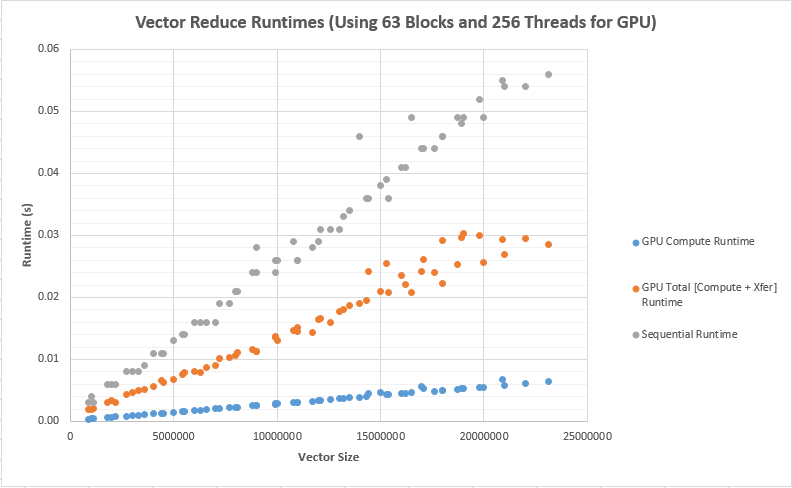
\includegraphics[width=.9\linewidth]{runtime_scatter}
    \caption{Runtimes for vector reduce (using a good number of GPU blocks/threads).}
    \label{fig:runtime_scatter}
  \end{figure}


  \begin{figure}[h]
    \centering
    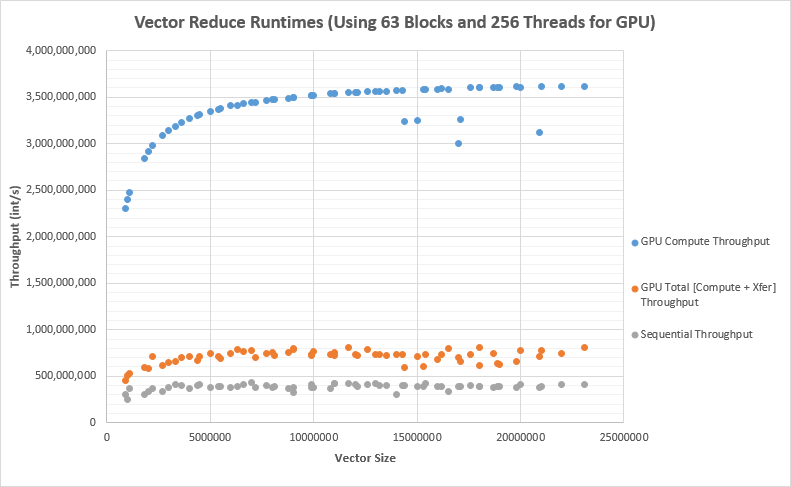
\includegraphics[width=.9\linewidth]{throughput_scatter}
    \caption{Runtimes for vector reduce (using a good number of GPU blocks/threads).}
    \label{fig:throughput_scatter}
  \end{figure}

  \begin{figure}[h]
    \centering
    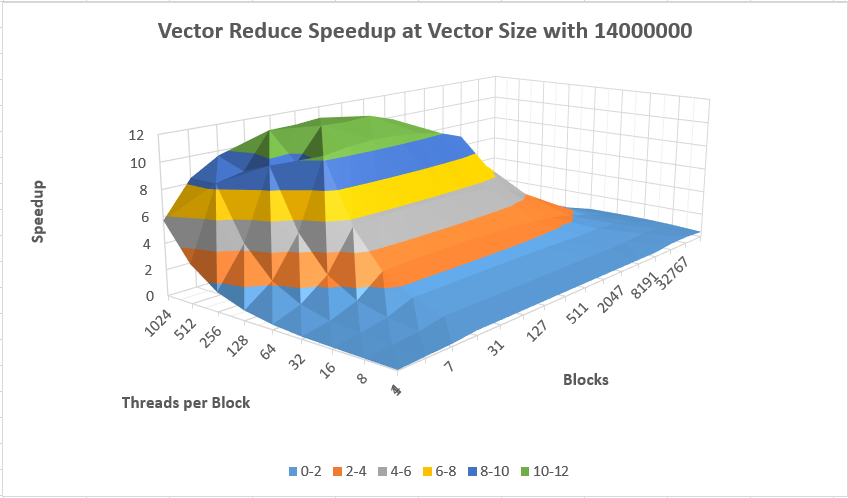
\includegraphics[width=.9\linewidth]{speedup_surface}
    \caption{A comparison of speedup for the computation portion of vector reduce across differing numbers of block and threads using a good vector size.}
    \label{fig:compute_speedup_surface}
  \end{figure}

  \begin{figure}[h]
    \centering
    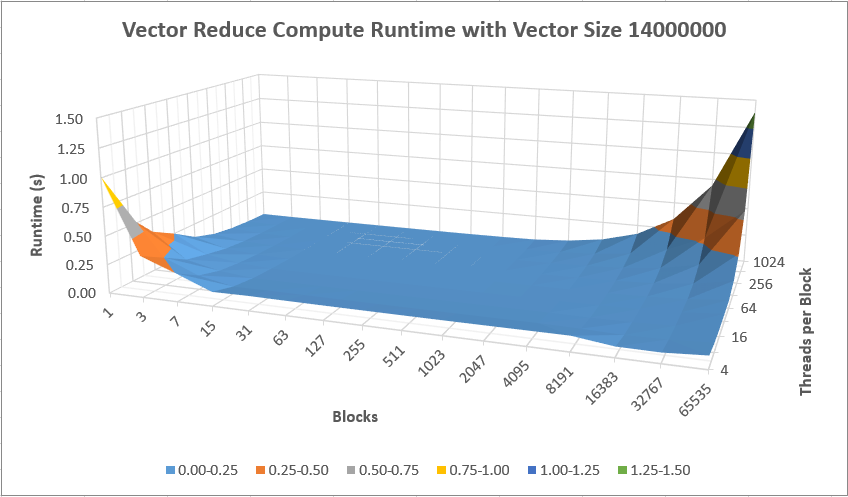
\includegraphics[width=.9\linewidth]{compute_runtime_surface}
    \caption{A comparison of runtime for the computation portion of vector reduce across differing numbers of block and threads using a good vector size.}
    \label{fig:compute_runtime_surface}
  \end{figure}

  \begin{figure}[h]
    \centering
    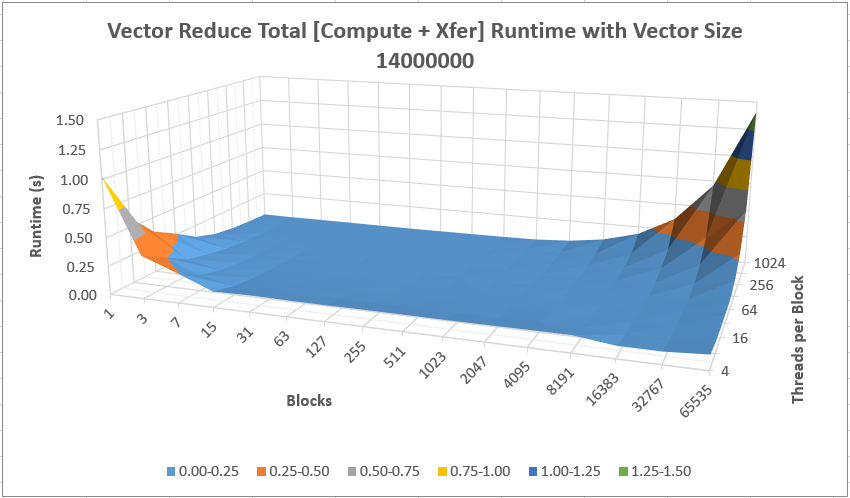
\includegraphics[width=.9\linewidth]{total_runtime_surface}
    \caption{A comparison of runtime for the computation and data transfer of vector reduce across differing numbers of block and threads using a good vector size.}
    \label{fig:total_runtime_surface}
  \end{figure}

  \begin{figure}[h]
    \centering
    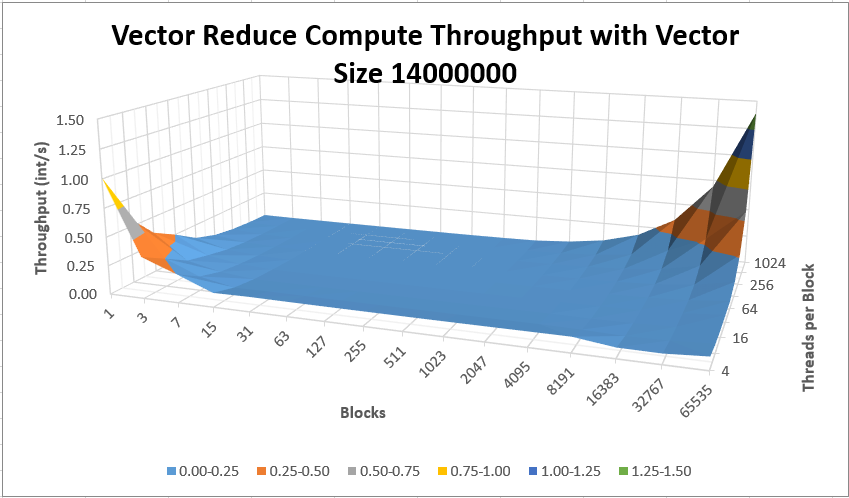
\includegraphics[width=.9\linewidth]{compute_throughput_surface}
    \caption{A comparison of throughput for the computation portion of vector reduce across differing numbers of block and threads using a good vector size.}
    \label{fig:compute_throughput_surface}
  \end{figure}

  \begin{figure}[h]
    \centering
    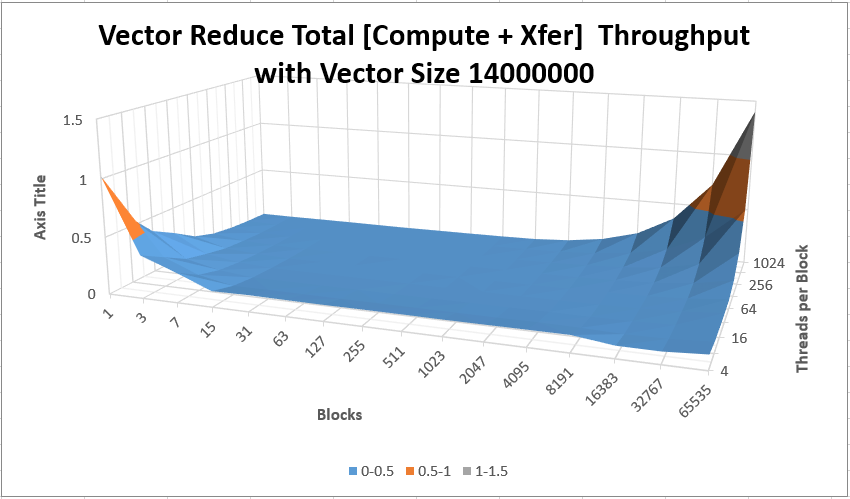
\includegraphics[width=.9\linewidth]{total_throughput_surface}
    \caption{A comparison of throughput for the computation and data transfer of vector reduce across differing numbers of block and threads using a good vector size.}
    \label{fig:total_throughput_surface}
  \end{figure}

\newpage
\section{Discussion}
\subsection{Speedups}
The speedups were lower than I would have expected, with a maximum speedup of around $11$. As usual, this was likely due to the weak GPU. However, we can still see where the best speedups occurred. It appears that the best speedup occurrs using around $128$ - $256$ threads with around $63$ - $255$ blocks. Note that there is a sharp dropoff in speed once more than $1024$ blocks are used due to the fact that this is when the reduction algorithm makes a significant change: intermediate kernel launches start to be used to reduce the vector enough (so that it has fewer elements than the maximum of threads per block) for the final kernel call to complete the reduction. Over using threads does seem to cause some reduction in performance, but not as significantly as overuse of blocks does.

\subsection{Data Transfer}
Data transfer was a small, but relatively uniform hindrance to performance. Interestingly enough, however, data transfer apears to play a smaller role in the runtime of the GPU reduction at larger vector sizes. It would be interesting to explore this further in an environment where GPU operations weren't limited to 2 seconds to see if the performance hit truly does level off.

\section{Issues}
\subsection{Windows Takes Away the GPU}
As I have stated before, Windows takes control of the GPU away from the program should a GPU operation take longer than $2$ seconds. While this does limit the range of vector sizes I am allowed to try, I believe I still acquire meaningful runs that demonstrate the necessary penomena.

\subsection{Weak GPU}
The weakness of the GPU makes it hard to demonstrate impressive performance.

\subsection{Ill Defined Assignment}
Not having specific guidelines made it somewhat difficult to complete the assignment on an appropriate timeline.

\subsection{Personal Folly}
I wanted to attempt using a personal algorithm where I divided the vector into shares for each block rather than simply striding the threads across the entire array. This became difficult to debug and likely would have reduced performance, so this strategy was abandoned (although much later than it should have been).
  
\end{document}